\chapter{GSAS-II and CIF}\index{CIF}\label{Chap:G2CIF}

\section{Introduction to CIF}
Work on CIF\index{CIF|textbf} began in the late 1980's as a mechanism to communicate small-molecule single-crystal crystallographic results from the International Union for Crystallography (IUCr). Indeed  entire short crystallographic articles could be placed in a CIF for submission to IUCr Journals. 
At that time CIF was an abbreviation for Crystallographic Information File, so a reference to a ``CIF file'' was a bit redundant. 

CIF is intended to be read and even edited by humans. The basic structure of CIF is that labels, known in CIF as data names, are associated with values, as shown in these examples: 
\begin{quote}
\texttt{\\
\_cell\_length\_c                  12.32318(8)\\
\_cell\_angle\_alpha               90.0\\
\_symmetry\_cell\_setting          orthorhombic\\
\_space\_group\_name\_H-M\_alt       'P 41 21 2'\\
\_computing\_structure\_refinement\\
;  GSAS-II (Toby, Brian H. \& Von Dreele, Robert B.;\\
Journal of Applied Crystallography 46, 544-549, 2013)\\
;\\
}    
\end{quote}
The above examples show inclusion of numerical values with and without a s.u. value, and several representations for character strings. Note that quotation marks are required when a string contains spaces, and the semicolon notation is used for strings that span multiple lines of text. The use of white space including line breaks is solely for the convenience of human readers. A single space serves the same purpose as multiple spaces and new-line characters are not distinguished from spaces for the purpose of parsing a file. 

To specify a series of values to be associated with a data name, the \texttt{loop\_}
keyword is used: 

\begin{quote}
\texttt{
loop\_ \_space\_group\_symop\_operation\_xyz \\
   'x, y, z'\\
   '-x, -y, z+1/2'\\
   '-y+1/2, x+1/2, z+1/4'\\
}    
\end{quote}
A table of values for several data names can also be created using the \texttt{loop\_}
keyword:

\begin{quote}
\texttt{
loop\_\\
   \_atom\_site\_type\_symbol\\
   \_atom\_site\_fract\_x\\
   \_atom\_site\_fract\_y\\
   \_atom\_site\_fract\_z\\
   Er        0.87730(5)    0.35493(5)    0.13550(5)\\
   Ge       0.90666(11)   0.15231(13)   0.61955(12)\\
}
\end{quote}

There are two special placeholder values used in CIF. A value of ``?'' (a question mark, which may be used without quotes) indicates that a value is unknown or is unspecified. 
A value of ``.'' (a period, which may also be used without quotes) indicates that the data name
does not have an appropriate in the specified context. 

CIFs are organized in blocks, where each block is an independent collection of data items and their values. 
Note that the beginning of a block is indicated by an name that begins with the string \texttt{data\_}, but the name that follows the underscore is considered arbitrary and may be changed when the CIF is archived. This is not a complete guide to the syntax of CIF, but this should provide a good overview as to what is required. 

CIF was unusual when created, if not unique, in that every CIF data name was given a formal and permanent definition in a set of documents called the CIF data dictionaries. Should a definition need to be changed, a new CIF data name is coined. 

By the mid-1990's, the utility of CIF had been demonstrated and work was began to develop CIF data dictionaries for applications beyond small-molecule crystallography. As this was done, CIF was renamed as the Crystallographic Information Framework\index{Crystallographic Information Framework|textbf}, as CIF was taking on the role of becoming a formal language for communication of crystallography, not just a file format. This also has the benefit that the term ``CIF file'' was no longer a redundancy. 

The pdCIF dictionary, with definitions for many items needed for powder diffraction, was one of the first to be started and took me the better part of a decade. One of the major problems was that a data name can only be associated with a single value or a single series of values within a CIF block. 
That rule means that, for example, lattice parameters can only be defined once in a block. 
Thus, to report a powder refinement with two crystallographic phases, a separate block would be needed for each phase. A mechanism was developed for pdCIF to establish logical connections between CIF blocks. Another reason that this project took so long was that, as it progressed, more stringent rules were created for the CIF data dictionary to enforce database conventions, so completed work sometimes needed revisions. 

CIF has been a major success story. 
For at least a decade, CIF has been \textit{the} universal standard for communication of crystallographic information.
Most journals require deposition of crystallographic results in CIF for electronic archival. Better journals require deposition of a CIF that includes the data used for the fit and documents the analysis process.
I frequently hear people use the term CIF as a synonym for a crystal structure. To the best of my knowledge, the only other field that has been as successful as crystallography in sharing data has been astronomy, but astronomers do have the advantage that they are all looking at the same specimen (the sky).

\section{GSAS-II CIF Imports}
GSAS-II is able to import phase information, single-crystal structure factors and powder diffraction data from CIFs. This is done from the menus associated with data imports (as discussed in \ref{Chap:ImportExport}. CIFs are parsed using the Python pyCifRW package from James Hester\index{Hester, J.}. James also leads the IUCr committee that oversees CIF development, so it may come as no surprise that pyCifRW requires that a CIF have correct syntax in order to be read. Databases do contain non-compliant CIFs and there is some software is reasonably tolerant of syntax errors. Should you encounter a CIF that GSAS-II will not read, you are recommended to use the free CCDC enCIFer program (\url{https://www.ccdc.cam.ac.uk/solutions/software/encifer/})\index{software!enCIFer|textbf}, which can help you locate and fix CIF syntax errors. There are several other programs that can do this, but I am not familiar with any. You might also have success with asking an AI agent, such as CoPilot or Gemini to examine and correct the file for syntax errors. 

One special type of CIF processing takes place when files created on the ISODISTORT\index{software!ISODISTORT} web site are imported, as will be discussed in \S\ref{ref:ISODISTORTcif}. These contain special CIF data items that describe how atomic parameters are set from representational analysis\index{representational analysis} modes. 

While reading of CIFs is a fairly complex task, as there is considerable complexity in how data may be organized in them, the importers function largely without any need for additional input, provided that the CIF has been properly written. One provides a file name, potentially selects which block(s) contain the desired data, when a choice is needed, and GSAS-II will then have the ingested the phase or histogram. 

\section{GSAS-II CIF Exports}

GSAS-II provides two forms of CIF files, which could be characterized as ``quick-and-dirty'' and ``comprehensive.'' The former type of CIFs are intended for communication of information between software programs and are used as would be any other exporter. One selects the exporter, selects a phase or histogram and the file is written. The process of creating a comprehensive CIF report from a GSAS-II project can be a much more complex task. The reason for this is that there is considerable information that the IUCr recommends for inclusion in a deposited CIF that you would need to supply. The CIF exporter will help you provide this information. Importantly, this information is placed into template files so that should the refinement be updated and the CIF then needs to be regenerated, the templates are reused and no additional work is needed. Since some of the information that is placed in the template files is likely to be useful for other projects, these files can be reused.

\subsection{Project CIF Exports}
When a Rietveld refinement contains a single histogram and a single phase, the entire CIF to document this can be a single CIF block. However, when more than one histogram or phase is used, then the CIF must have multiple blocks. When this is the case, GSAS-II will write a CIF block for each phase and a block for each histogram and finally a summary block that provides links between all the CIF blocks. 
Each CIF block is identified with a block tag. This block tag is intended to be completely unique and contains a timestamp, the CIF author name and the instrument name as well as the name of the project. If you include the institution name with the instrument, as well as use your name, it becomes quite unlikely that anyone else will duplicate the block tags. 

\begin{figure}
    \centering
    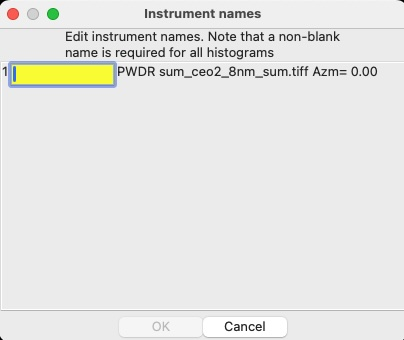
\includegraphics[width=0.35\linewidth]{figures/cif0.jpg}
    \caption{Project CIF generation: Opening window to enter instrument name(s), if any are blank.}
    \label{fig:cif0}
\end{figure}

\begin{figure}
    \centering
    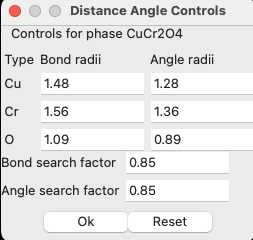
\includegraphics[width=0.3\linewidth]{figures/cif1.jpg}
    \caption{Project CIF generation: Select bond distance and angle search radii.}
    \label{fig:cif1}
\end{figure}

The process of writing a comprehensive CIF is outlined here. When the menu command for a project-based CIF export is first entered, you will first be asked to supply a name for the file to be written. 

Every powder histogram must have an instrument name supplied, since this is used to make the block tags unique. (This name can be edited on the histogram's ``Sample Parameters'' data tree entry.) If any are blank, the window shown in Fig. \ref{fig:cif0} is seen. 

You will then be asked to supply atomic radii for each phase, as seen in Fig. \ref{fig:cif1}. These are used to search for bond distances and angles that will be reported; the defaults for these values will probably be fine, but should you find that important distances are not being computed, it will be simple enough to include change these values later so that more (or fewer) values are generated. These radii values are saved in the project, so you will not be presented with these window(s) again. Once this has been completed, the main window for CIF generation is shown as in as seen in Fig. \ref{fig:cifmain}.

\begin{figure}
    \centering
    \begin{subfigure}{0.45\textwidth}
        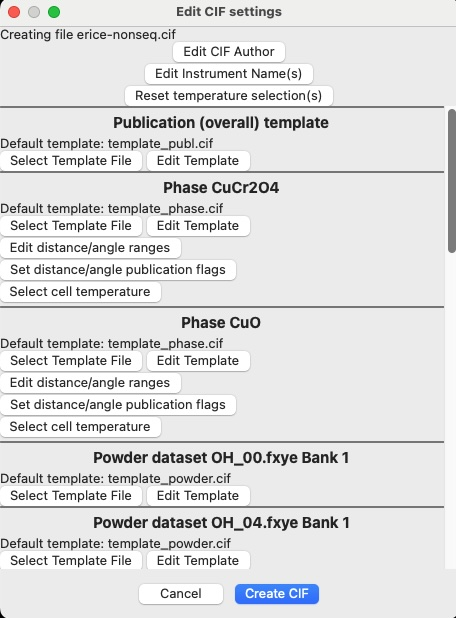
\includegraphics[width=0.9\linewidth]{figures/cif2.jpg}
        \caption{Example with multiple phases and histograms.}
        \label{fig:cifmainA} 
    \end{subfigure}
    \begin{subfigure}{0.45\textwidth}
        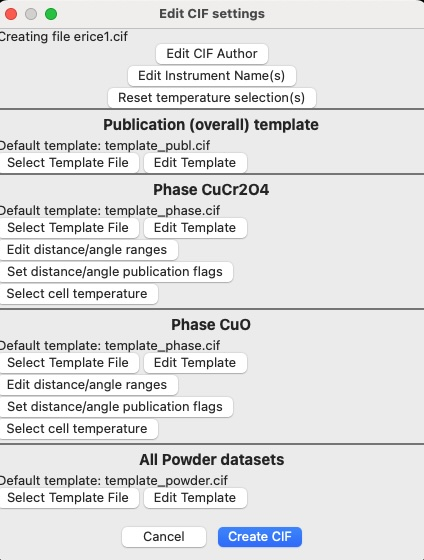
\includegraphics[width=0.9\linewidth]{figures/cif3.jpg}
        \caption{Multi-phase sequential fit example. Note that, unlike \ref{fig:cifmainA}, there is only a single entry for all histograms.}
    \end{subfigure}
    \caption{The main window for project CIF generation showing the difference between a multi-phase and multi-histogram example and for a sequential fit. For the latter, the histograms are assumed to have the same metadata and only one need be edited. Should problems be noted with the project,
    for example that data collection temperatures appear to be at default values, the top
    of the window note this and will have a button to show warnings.}
    \label{fig:cifmain} 
\end{figure}

Setting the CIF author name is strongly recommended, since this is also used to make the block tags unique. For a multi-histogram export, the ``Edit Instrument Name(s)'' button will open the window seen in Fig. \ref{fig:cif4}. Note that the ``down arrow'' button allows a value to be copied to all the entries below, so the instrument name only needs to be entered once. In a sequential refinement, the instrument names must be the same, and only the first value is shown. 

\begin{figure}
    \centering
    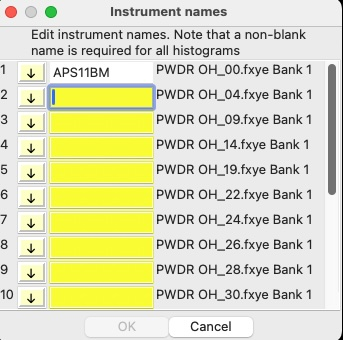
\includegraphics[width=0.35\linewidth]{figures/cif4.jpg}
    \caption{Project CIF generation: Set instrument name. The ``down arrow'' button copies the value to all the histograms below. The yellow background indicates that a blank value is invalid for those entries.}
    \label{fig:cif4}
\end{figure}

In the main CIF creation window (as seen in Fig. \ref{fig:cifmain}), there are buttons in each section that reference a CIF template. There are three types of templates, for the overall project, for phases and for histograms, where the fields in the template are taken from IUCr guidelines for reporting powder diffraction results (\url{https://journals.iucr.org/services/cif/powder.html}). An example of the window that appears when a template is edited is shown in Fig. \ref{fig:cif5a}. As will be clear from looking at these items, they describe the instrument used for data collection. This is likely to be the same for every CIF generated with this instrument, so considerable time will be saved by reusing this content once the template is prepared. Save the template file before pressing the ``Use'' button and the next time that a CIF is prepared, you can read the saved template file in place of the default. Note two features of this template window. There is a ``help button'' (labeled with a question mark; on Windows this appears in yellow) for every CIF data name that has a definition in the CIF dictionaries that are provided as part of the GSAS-II installation. Pressing the help button causes the definition to be shown, as seen in Fig. \ref{fig:cif5b}. Also, the data entry boxes in this window can be resized by dragging the right-angle symbol in the lower right of the data entry box. Increasing this size is helpful when lengthy values will be entered. This is also shown in Fig. \ref{fig:cif5b}.

\begin{figure}
    \centering
    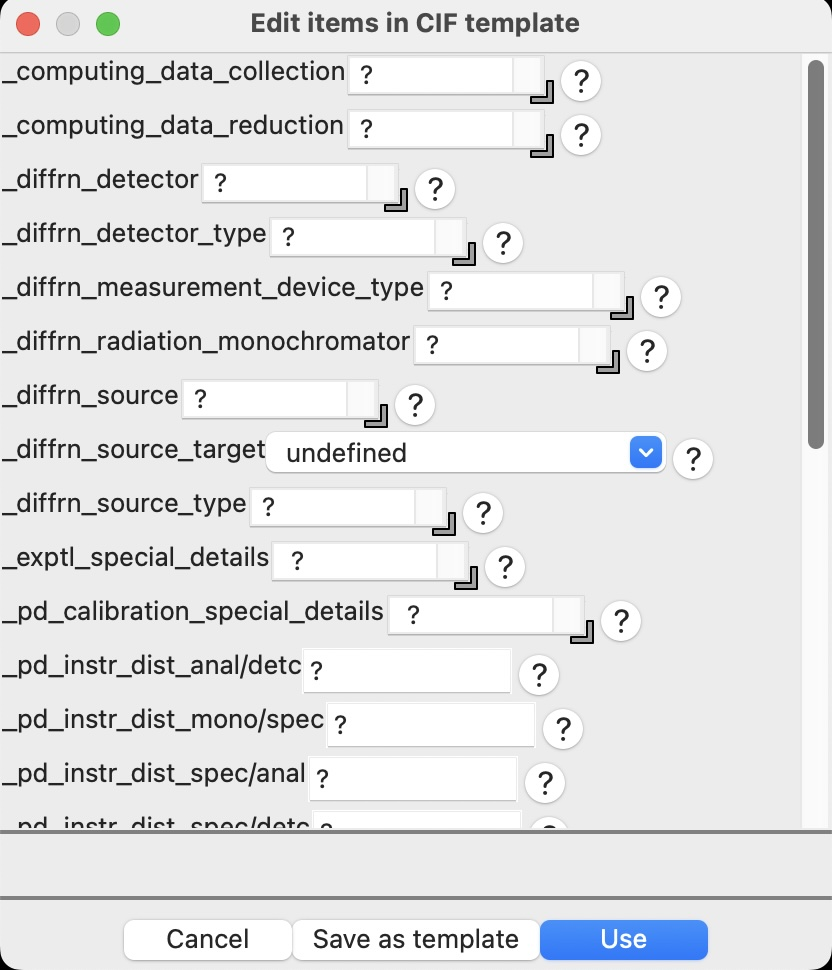
\includegraphics[width=0.4\linewidth]{figures/cif5a.jpg}
    \caption{Editing a CIF template for project CIF generation. This shows the default contents for the histogram template.}
    \label{fig:cif5a}
\end{figure}

\begin{figure}
    \centering
    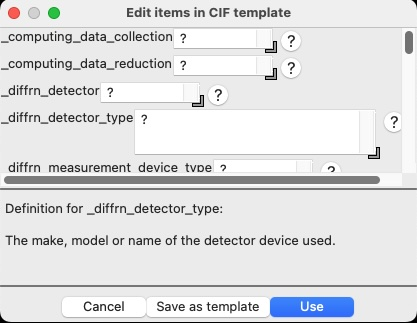
\includegraphics[width=0.4\linewidth]{figures/cif5b.jpg}
    \caption{Editing a CIF template for project CIF generation. The help button (with a question mark) has been pressed for the \texttt{\_diffrn\_detector\_type} entry and the definition information from the CIF dictionary is shown below. Also, the ``angle bracket'' at the lower right of the data entry widget for that CIF item has been used to increase the size of that box.}
    \label{fig:cif5b}
\end{figure}

Associated with each phase is a table of bond distances and angles; each value in that table has a ``publish'' flag. IUCr Journals will generate tables from this information, but will only include the values that have been flagged with the ``publish'' flag set as true (which is the default). The ``Set distance/angle publication flags'' window, where an example is shown as \ref{fig:cif6}. This window serves two purposes. The publication flags can be set here, though I think this is commonly not done anymore. More significantly, you can see if the radii are set in the right range to pick up the desired distances and angles, but not non-bonding contacts, unless they are of interest. In the example shown here, the desired bond distances were found, but the angle radii needed to be lengthened so that the bond angles were included.

\begin{figure}
    \centering
    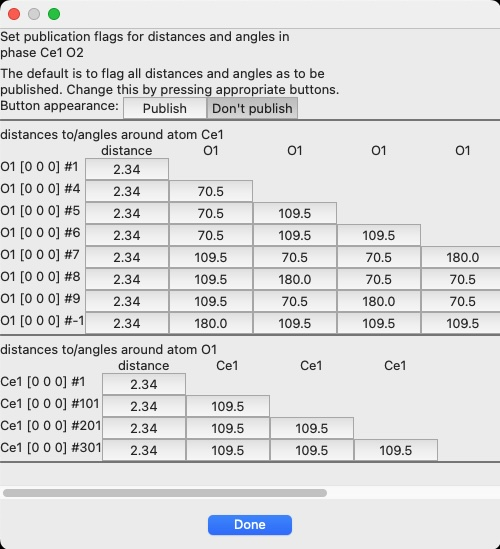
\includegraphics[width=0.6\linewidth]{figures/cif6.jpg}
    \caption{An example of the bond distance and angle window from CIF generation. Note that this phase as no refined coordinates, so no uncertainties are included here. Normally, distances and angles would be have s.u. values in crystallographic notation.}
    \label{fig:cif6}
\end{figure}

When the CIF has been customized by entering information into the templates, atomic radii and distance/angle flags, press the ``Create CIF'' button and the CIF will be created. Note that all this customization information is saved in the GSAS-II project (\texttt{.gpx}) file. This means that if the project export CIF menu command is used again, the revised CIF will retain all of the information you entered, but the cell dimensions, coordinates, distances, etc. will all be updated. Thus, all the work invested in creating a well-documented CIF will not be wasted should the refinement be updated. 

\section{For More Information}

\begin{itemize}
\item 
  \textit{International Tables for Crystallography, Volume G: Definition and exchange of crystallographic data} (2006). Hall, S. R., \& McMahon, B. (Eds.). DOI: 10.1107/97809553602060000107. 
  \begin{quote}
  This is the canonical reference for CIF. A revised edition is currently being prepared (2026). Volume G includes a chapter on powder diffraction and another on pdCIF. If your library does not have a physical copy of this, they may offer on-line access.
  \end{quote}

\item 
  ``Use of CIF for powder diffraction data,'' Chapter 4.10. (2019) B. H. Toby, in \textit{International Tables for Crystallography, Volume H: Powder Diffraction}, edited by C. J. Gilmore, J. A. Kaduk, and H. Schenk, DOI: 10.1107/97809553602060000889
  \begin{quote}
A shorter and less comprehensive introduction to pdCIF is available in this volume. Again, if your library does not have a physical copy of this, they may offer on-line access.
  \end{quote}

\item 
  There is a considerable amount of information on CIF, including nicely formatted versions of the various CIF dictionaries, on the IUCr website at \url{https://www.iucr.org/resources/cif}.

\end{itemize}
